%Version 2.1 April 2023
% See section 11 of the User Manual for version history
%
%%%%%%%%%%%%%%%%%%%%%%%%%%%%%%%%%%%%%%%%%%%%%%%%%%%%%%%%%%%%%%%%%%%%%%
%%                                                                 %%
%% Please do not use \input{...} to include other tex files.       %%
%% Submit your LaTeX manuscript as one .tex document.              %%
%%                                                                 %%
%% All additional figures and files should be attached             %%
%% separately and not embedded in the \TeX\ document itself.       %%
%%                                                                 %%
%%%%%%%%%%%%%%%%%%%%%%%%%%%%%%%%%%%%%%%%%%%%%%%%%%%%%%%%%%%%%%%%%%%%%

%%\documentclass[referee,sn-basic]{sn-jnl}% referee option is meant for double line spacing

%%=======================================================%%
%% to print line numbers in the margin use lineno option %%
%%=======================================================%%

%%\documentclass[lineno,sn-basic]{sn-jnl}% Basic Springer Nature Reference Style/Chemistry Reference Style

%%======================================================%%
%% to compile with pdflatex/xelatex use pdflatex option %%
%%======================================================%%

%%\documentclass[pdflatex,sn-basic]{sn-jnl}% Basic Springer Nature Reference Style/Chemistry Reference Style


%%Note: the following reference styles support Namedate and Numbered referencing. By default the style follows the most common style. To switch between the options you can add or remove �Numbered� in the optional parenthesis. 
%%The option is available for: sn-basic.bst, sn-vancouver.bst, sn-chicago.bst, sn-mathphys.bst. %  
 
%%\documentclass[sn-nature]{sn-jnl}% Style for submissions to Nature Portfolio journals
%%\documentclass[sn-basic]{sn-jnl}% Basic Springer Nature Reference Style/Chemistry Reference Style
\documentclass[sn-mathphys,Numbered]{sn-jnl}% Math and Physical Sciences Reference Style
%%\documentclass[sn-aps]{sn-jnl}% American Physical Society (APS) Reference Style
%%\documentclass[sn-vancouver,Numbered]{sn-jnl}% Vancouver Reference Style
%%\documentclass[sn-apa]{sn-jnl}% APA Reference Style 
%%\documentclass[sn-chicago]{sn-jnl}% Chicago-based Humanities Reference Style
%%\documentclass[default]{sn-jnl}% Default
%%\documentclass[default,iicol]{sn-jnl}% Default with double column layout

%%%% Standard Packages
%%<additional latex packages if required can be included here>

\usepackage{graphicx}%
\usepackage{multirow}%
\usepackage{amsmath,amssymb,amsfonts}%
\usepackage{amsthm}%
\usepackage{mathrsfs}%
\usepackage[title]{appendix}%
\usepackage{xcolor}%
\usepackage{textcomp}%
\usepackage{manyfoot}%
\usepackage{booktabs}%
\usepackage{algorithm}%
\usepackage{algorithmicx}%
\usepackage{algpseudocode}%
\usepackage{listings}%
\usepackage{accents}%
%%%%

%%%%%=============================================================================%%%%
%%%%  Remarks: This template is provided to aid authors with the preparation
%%%%  of original research articles intended for submission to journals published 
%%%%  by Springer Nature. The guidance has been prepared in partnership with 
%%%%  production teams to conform to Springer Nature technical requirements. 
%%%%  Editorial and presentation requirements differ among journal portfolios and 
%%%%  research disciplines. You may find sections in this template are irrelevant 
%%%%  to your work and are empowered to omit any such section if allowed by the 
%%%%  journal you intend to submit to. The submission guidelines and policies 
%%%%  of the journal take precedence. A detailed User Manual is available in the 
%%%%  template package for technical guidance.
%%%%%=============================================================================%%%%

%\jyear{2021}%

%% as per the requirement new theorem styles can be included as shown below
\theoremstyle{thmstyleone}%
\newtheorem{theorem}{Theorem}%  meant for continuous numbers
%%\newtheorem{theorem}{Theorem}[section]% meant for sectionwise numbers
%% optional argument [theorem] produces theorem numbering sequence instead of independent numbers for Proposition
\newtheorem{proposition}[theorem]{Proposition}% 
%%\newtheorem{proposition}{Proposition}% to get separate numbers for theorem and proposition etc.

\theoremstyle{thmstyletwo}%
\newtheorem{example}{Example}%
\newtheorem{remark}{Remark}%

\theoremstyle{thmstylethree}%
\newtheorem{definition}{Definition}%

\DeclareMathOperator*{\argmax}{arg\,max}
\DeclareMathOperator*{\argmin}{arg\,min}

\raggedbottom
%%\unnumbered% uncomment this for unnumbered level heads

\begin{document}

\title[Topological k-means]{Topological k-means: a graph-based algorithm for data clustering using geodesic distances}

%%=============================================================%%
%% Prefix	-> \pfx{Dr}
%% GivenName	-> \fnm{Joergen W.}
%% Particle	-> \spfx{van der} -> surname prefix
%% FamilyName	-> \sur{Ploeg}
%% Suffix	-> \sfx{IV}
%% NatureName	-> \tanm{Poet Laureate} -> Title after name
%% Degrees	-> \dgr{MSc, PhD}
%% \author*[1,2]{\pfx{Dr} \fnm{Joergen W.} \spfx{van der} \sur{Ploeg} \sfx{IV} \tanm{Poet Laureate} 
%%                 \dgr{MSc, PhD}}\email{iauthor@gmail.com}
%%=============================================================%%

\author*[1]{\fnm{Alexandre L. M} \sur{Levada}}\email{alexandre.levada@ufscar.br}

\author[1]{\fnm{Ant\^onio C. A. de} \sur{Azevedo}}\email{azevedoantonio@estudante.ufscar.br}
%\equalcont{These authors contributed equally to this work.}

\author[2]{\fnm{Fernando} \sur{Borges}}\email{fernando.borges@estudante.ufscar.br}
%\equalcont{These authors contributed equally to this work.}

\affil*[1]{\orgdiv{Computing Department}, \orgname{Federal University of S\~ao Carlos}, \orgaddress{\street{Rod. Washington Luis, km. 235}, \city{S\~ao Carlos}, \postcode{13565-905}, \state{SP}, \country{Brazil}}}

\affil[2]{\orgdiv{Statistics Department}, \orgname{Federal University of S\~ao Carlos}, \orgaddress{\street{Rod. Washington Luis, km. 235}, \city{S\~ao Carlos}, \postcode{13565-905}, \state{SP}, \country{Brazil}}}

%\affil[2]{\orgdiv{Department}, \orgname{Organization}, \orgaddress{\street{Street}, \city{City}, \postcode{10587}, \state{State}, \country{Country}}}
%
%\affil[3]{\orgdiv{Department}, \orgname{Organization}, \orgaddress{\street{Street}, \city{City}, \postcode{610101}, \state{State}, \country{Country}}}

%%==================================%%
%% sample for unstructured abstract %%
%%==================================%%

\abstract{Clustering is one of the most important tasks in machine learning and data science. Several clustering algorithms have been proposed to mitigate limitations from unsupervised learning in pattern recognition. However, clustering high dimensional data is still a challenge. In this paper, we propose topological k-means, a graph-based method for data clustering that uses the Dijkstra algorithm to compute geodesic distances between sample points in the discrete approximate data manifold. Moreover, the computational complexity of the proposed algorithm is reasonably low in comparison to modern clustering techniques, as it is linear in the number of samples and also in the number of edges of the k-NN graph. Computational experiments with real datasets show that the proposed method is capable of improving the quality of the obtained clusters in terms of external validity measures in comparison to regular k-means and a state-of-the-art approach, the HDBSCAN algorithm, defining a viable and promissing alternative to existing clustering algorithms.}

%%================================%%
%% Sample for structured abstract %%
%%================================%%

% \abstract{\textbf{Purpose:} The abstract serves both as a general introduction to the topic and as a brief, non-technical summary of the main results and their implications. The abstract must not include subheadings (unless expressly permitted in the journal's Instructions to Authors), equations or citations. As a guide the abstract should not exceed 200 words. Most journals do not set a hard limit however authors are advised to check the author instructions for the journal they are submitting to.
% 
% \textbf{Methods:} The abstract serves both as a general introduction to the topic and as a brief, non-technical summary of the main results and their implications. The abstract must not include subheadings (unless expressly permitted in the journal's Instructions to Authors), equations or citations. As a guide the abstract should not exceed 200 words. Most journals do not set a hard limit however authors are advised to check the author instructions for the journal they are submitting to.
% 
% \textbf{Results:} The abstract serves both as a general introduction to the topic and as a brief, non-technical summary of the main results and their implications. The abstract must not include subheadings (unless expressly permitted in the journal's Instructions to Authors), equations or citations. As a guide the abstract should not exceed 200 words. Most journals do not set a hard limit however authors are advised to check the author instructions for the journal they are submitting to.
% 
% \textbf{Conclusion:} The abstract serves both as a general introduction to the topic and as a brief, non-technical summary of the main results and their implications. The abstract must not include subheadings (unless expressly permitted in the journal's Instructions to Authors), equations or citations. As a guide the abstract should not exceed 200 words. Most journals do not set a hard limit however authors are advised to check the author instructions for the journal they are submitting to.}

\keywords{Clustering, k-means, HDBSCAN, high dimensional data, geodesic distance}

%%\pacs[JEL Classification]{D8, H51}

%%\pacs[MSC Classification]{35A01, 65L10, 65L12, 65L20, 65L70}

\maketitle

\section{Introduction}\label{sec1}

Machine learning has witnessed unprecedented growth in recent years, and within this expansive domain, data clustering stands out as a pivotal technique with profound implications for data analysis and pattern recognition \cite{Clustering1,Clustering2,Clustering3}. Clustering, in the domain of machine learning, is a technique that involves grouping similar data points together, based on certain inherent characteristics, without the need for predefined labels. The fundamental premise underlying clustering is the identification of natural groupings or patterns within data, which facilitates a more nuanced understanding of the underlying structure \cite{Clustering4}. This unsupervised learning approach has far-reaching applications across various domains, including image processing, pattern recognition, and data mining \cite{Clustering5}.

The most popular clustering method is k-means, a partitional algorithm, which aim to divide a dataset into $k$ distinct, non-overlapping subgroups or clusters by minimizing the sum of squared distances between data points and the centroid of their assigned cluster \cite{kmeans1,kmeans2}. The main advantages of k-means are: 1) computational efficiency, as it is linear in the number of samples, making it suitable for large datasets; and 2) simplicity and versatility, as it is easy to implement and applicable in various domains, as it can hadle different types of data. However, k-means also has several limitations, among which we can cite: 1) as it relies on the Euclidean distance, it suffers from a kind of non-spherical blindness and high sensitivity to outliers in data; and 2) it struggles with clusters with varying densities and shapes. 

Modern clustering algorithms are often capable of overcoming some limitations of k-means. Hierarchical Density-Based Spatial Clustering of Applications with Noise, or simply HDBSCAN, is an advanced clustering algorithm that extends the capabilities of traditional density-based methods, such as DBSCAN \cite{HDBSCAN}. The key innovation lies in its ability to discover clusters of varying shapes and densities in a dataset while being robust to noise. HDBSCAN operates by constructing a hierarchical clustering tree and then extracting stable and significant clusters from this structure \cite{HDBSCAN*}. The main advantages of HDBSCAN are: 1) noise handling, as it explicitly identifies and labels noise points, providing a clear distinction between valid clusters and noise in the data; 2) flexibility in cluster shapes, as it is not constrained by assumptions about the shape or size of clusters, making it suitable for datasets with complex structures; and 3) adaptability to different densities, as it adapts well to clusters with varying densities, making it particularly effective in scenarios where clusters exhibit different levels of compactness. On the ohter hand, the main limitations of HDBSCAN are \cite{HDBSCAN_}: 1) computational complexity, as it is an intensive algorithm, especially for large datasets; 2) sensitivity to parameters, as the performance can be significantly influenced by tuning its parameters; and 3) limited for global structure, as it focuses on local density structures, and while it is excellent for identifying microclusters. Another issue with HDBSCAN is related to performance and approximation. For huge datasets, a random sample for k-means can get a good approximation of the overall result. But for HDBSCAN, it's not clear how to evaluate it in subsets of the data.

Despite many advances, one open problem in clustering is how to deal with high dimensional data, that is, situations in which the number of features $m$ is order of magnitudes larger than the number of samples $n$ \cite{cluster_high_dim_1,cluster_high_dim_2,cluster_high_dim_3}. To tackle this problem, we propose topological k-means, or simply top k-means, a graph-based algorithm that computes geodesic distances between samples in the data manifold using Dijkstra's algorithm. Basically, the ideia is to approximate the data manifold by a k-NN graph and then use the length of the shortest paths as an approximation to the underlying geodesic distances. The main contributions of this paper are twofold: 1) after building a graph representation and replacing the Euclidean distances by the geodesic distances, topological k-means is able to detect clusters with different shapes, depending on the graph topology; and 2) topological k-means avoids the lack of discriminating power of the Euclidean distance in high dimensional spaces, producing meaningful clusters even when the number of features $m$ is much larger than the number of samples $n$ (the curse of the dimensionality).

The remaining of the paper is organized as follows: Section 2 presents an overview of the k-means clustering algorithm. Section 3 discusses Dijkstra's algorithm in detail, showing that is always returns the geodesic distances in graphs whose edge weights are positive. Section 4 describes the proposed topological k-means algorithm, explaining how it works and analyzing its computational complexity. Section 5 shows the computational experiments with regular k-means, topological k-means and HDBSCAN, presenting the obtained results in terms of three external cluster quality mesures: Rand index, normalized mutual information index and V-measure. Finally, Section 6 presents our conlcusions and final remarks.

\section{The k-means clustering algorithm}

The k-means algorithm is an unsupervised method in the sense that learning is completely autonomous. Its first version was originally proposed in 1957 by Stuart P. Loyd in the context of pulse code modulation, but only published decades later, in 1982 \cite{Loyd}. The basic idea of k-means consists in grouping points according to a similarity measure, with the obtained results (clusters) strongly depending on the similarity measure chosen. In its regular version, k-means adopts the Euclidean distance, which makes the algorithm ``blind'' for non spherical clusters.

The problem formulation is as follows: given a data matrix $X^T = \{ \vec{x}_1, \vec{x}_2, ..., \vec{x}_n \}$, where $\vec{x}_i \in R^d$, the objective is to partition $X$ in $k < n$ groups or clusters in order to minimize the intra-cluster scattering, that is, to find the optimal partition $S^{*} = \{ s_1^{*}, s_2^{*}, ..., s_k^{*} \}$ that satisfies the following criterion, also known as within-cluster sum of the squares (WCSS) \cite{kmeans_survey}:

\begin{equation}
	S^{*} = \argmin_{S} \sum_{i=1}^{k} \sum_{\vec{x} \in s_i} \lVert \vec{x} - \vec{\mu}_i  \rVert^2
\end{equation} where $k$ denotes the number of partitions and $\vec{\mu}_i$ is the centroid of partition set $s_i$. Note that, intuitively, the objective function determines that we must make the centroid of each partition be as close as possible to the data points that define that partition.

It has been shown that finding the optimal solution to this problem is NP-Hard for any number of dimensions $d$ (even two dimensions). The heuristic adopted by k-means to simplify the problem and hence lead to a polynomial time algorithm, consists of fixing the value of $k$. Therefore, the parameter $k$ (number of clusters) must be chosen before the algorithm is executed, what is unknown is some situations. In the following, we present two major results that help us better understand the k-means algorithm.

\vspace{0.5cm}
\begin{theorem}
	Given a non-empty cluster $s_k$, its centroid or mean is the only choice of center which minimizes internal scattering
	\begin{equation}
		WS(\vec{c}^{(k)}) = \sum_{\vec{x} \in s_k} \lVert \vec{x} - \vec{c}^{(k)}  \rVert^2
	\end{equation}
\end{theorem}

First, note that:

\begin{equation}
	WS(\vec{c}^{(k)}) = \sum_{\vec{x} \in s_k} \lVert \vec{x} - \vec{c}^{(k)}  \rVert^2 = \sum_{\vec{x} \in s_k} ( \vec{x} - \vec{c}^{(k)} )^T ( \vec{x} - \vec{c}^{(k)} )
\end{equation}

Applying the distributive, we have:

\begin{equation}
	WS(\vec{c}^{(k)}) = \sum_{\vec{x} \in s_k} \left( \vec{x}^T \vec{x} - 2 \vec{x}^T \vec{c}^{(k)} + {\vec{c}^{(k)}}^{T} \vec{c}^{(k)}  \right)
\end{equation}

The necessary condition for the minimization is:

\begin{equation}
	\frac{\partial}{\partial \vec{c}^{(k)}} WS(\vec{c}^{(k)}) = 0
\end{equation} which leads to:

\begin{equation}
	2 \sum_{\vec{x} \in s_k} \vec{x} - 2 \sum_{\vec{x} \in s_k} \vec{c}^{(k)} = 0
\end{equation} whose solution is:

\begin{equation}
	\vec{c}^{(k)} = \frac{1}{n_k} \sum_{\vec{x} \in s_k} \vec{x}
\end{equation} where $n_k$ is the number of samples in the $k$-th cluster. The following result shows that the nearest centroid rule, that is, assign each data point $\vec{x}$ to the cluster whose center is the closest, produces an optimal solution to the k-means clustering problem.

\vspace{0.5cm}
\begin{theorem}
	Given a set $X$ of data points and a sequence of $k$ centroids $\vec{c}^{(1)}, \vec{c}^{(2)}, ..., \vec{c}^{(k)}$ a partition into clusters minimize the objective function 
	\begin{equation}
		\sum_{i=1}^{k} \sum_{\vec{x} \in s_i} \lVert \vec{x} - \vec{\mu}_i  \rVert^2
	\end{equation} if the algorithm assigns each sample $\vec{x}$ to the cluster $s_i$ with the closest centroid. 
\end{theorem}
\vspace{0.5cm}

The proof is trivial, since each sample $\vec{x}$ contributes exactly a single time to the sum defined by the previous objective function and when choosing to assign $\vec{x}$ to the cluster whose centroid is the closest, we clearly minimize the contribution to the objective function. Algorithm \ref{kmeans_algo} illustrates the pseudo-code of the k-means clustering method.

\begin{algorithm}[H]
\caption{k-means clustering algorithm}\label{kmeans_algo}
\begin{algorithmic}
\State // Parameters:
\State // $X$: the $n \times d$ data matrix (each row is a sample)
\State // $n$: the number of samples
\State // $k$: the number of clusters
\Function{k-means}{$X, n, k$}
\State $\vec{s}_1, \vec{s}_2, .., \vec{s}_k \gets select\_random\_seeds(X, k)$	\Comment{Select k random centers}
\For{$i \gets 1$; $i \leq k$; $i++$}	
	\State $\vec{\mu}_i \gets \vec{s}_i$		
\EndFor
\While{not convergence}
	\For{$i \gets 1$; $i \leq k$; $i++$}
		\State $\omega_i \gets \{ \}$		\Comment{Begin with $k$ empty partitions}
	\EndFor
	\For{$i \gets 1$; $i \leq n$; $i++$}
		\State $j \gets \argmin_l \lVert \vec{\mu}_l - \vec{x}_i \rVert$   \Comment{Find nearest centroid}
		\State $\omega_j \gets \omega_j \cup \{ \vec{x}_i \} $	\Comment{Assign sample to the cluster}
	\EndFor
	\For{$i \gets 1$; $i \leq k$; $i++$}
		\State $\vec{\mu}_i \gets \frac{1}{\lvert \omega_i \rvert}\sum_{\vec{x} \in \omega_i} \vec{x}$ \Comment{Recalculate the centroids}
	\EndFor
\EndWhile 
\State \textbf{return} $\omega_1, \omega_2, ..., \omega_k$	
\EndFunction
\end{algorithmic}
\end{algorithm}

The convergence of the k-means algorithm is usually measured in three different ways: 1) the centroids of the newly formed clusters do not move or their movement is less than a threshold; 2) the data points remain in the same clusters; and 3) a maximum number of iterations is reached.

\subsection{Complexity analysis}

Basically, the computational complexity of the k-means algorithm essentially depends on the following factors: the number of samples $n$, the number of centers $k$, the number of features $d$ and the number of iterations for convergence $t$ (which is often unknown).

First, note that the select\_random\_seeds(X, k) function and the initial FOR loop (outside the while) are accomplished in $O(k)$.The critical part is executing the WHILE loop, which we will analyze next. To obtain the closest centroid, note that we must compare it against $k$ centroids. Knowing that $k$ Euclidean distances will be necessary for this and that, to calculate each distance, we have a cost of $O(d)$. Thus, to decide which centroid is the closest to a sample, the computational cost is $O(kd)$. As the process is repeated for all $n$ data points, we have a cost of $O(nkd)$. Finally, since this process is repeated for an unknown number $t$ of iterations, the total cost of the k-means algorithm is $O(tnkd)$, which is nevertheless linear in the number of samples, leading to a quite efficient algorithm.

\section{Geodesic distances in graphs}

The problem of finding geodesic distances in graphs is solved by the computation of shortest paths in weighted graphs. 

\vspace{0.5cm}
\begin{definition}
Given a weighted graph $G = (V, E, w)$, where $V$ is the set of vertices, $E$ is the set of edges and $w: E \rightarrow R^{+}$ is a weighting function  for the edges, the weight of a path $P = v_0 v_1 v_2 ... v_n$ is given by: 
\begin{equation}
	w(P) = \sum_{i=1}^{n} w(v_{i-1}, v_i)
\end{equation}
\end{definition}

The optimum path $P^{*}$ from $v_0$ to $v_n$ is a minimizer for $w(P)$, that is:

\begin{equation}
	P^{*} = \argmin_P w(P)
\end{equation} provided there is a path between $v_0$ and $v_n$, otherwise the cost of the path is infinite. In the following, we present a nice property of optimum paths.

\vspace{0.5cm}
\begin{theorem}
Let $G = (V, E, w)$ and $P = v_0 v_1 v_2 ... v_n$ the optimum path from $v_0$ to $v_n$. For $0 \leq i < j \leq n$, let $P' = v_i v_{i+1} ... v_j$ a subpath of $P$. Then, $P'$ is the optimum path from $v_i$ to $v_j$.
\end{theorem}
\vspace{0.5cm}

In other words, any subpath from an optimum path $P$ is also optimum. This result shows that dynamic programming can be applied in the solution of shortest path problems. Dijkstra's algorithm combines dynamic programming and a greedy strategy to solve shortest path problems in a computationally efficient way. First, we define the main variables used by Dijkstra's algorithm. 

\begin{itemize}
	\item $\lambda(v)$: length of the shortest path from the root $s$ to vertex $v$.
	\item $\pi(v)$: predecessor of vertex $v$ in the shortest path tree.
	\item $Q$: priority queue to store the vertices (the smaller $\lambda(v)$, the higher the priority).
\end{itemize}

The priority queue $Q$ has three basic primitives: 

\begin{itemize}
	\item Insert($Q$, $v$): insert a vertex $v$ at the end of $Q$.
	\item ExtractMin($Q$): remove from $Q$ the vertex having the smallest $\lambda(v)$.
	\item DecreaseKey($Q$, $v$, $\lambda(v)$: update the priority of vertex $v$ in $Q$.
\end{itemize} 

Given the above, Dijkstra's method for building shortest paths in weighted graphs is presented in Algorithm \ref{dijkstra_algo} \cite{Cormen}.

\begin{algorithm}[H]
\caption{Dijkstra's algorithm}\label{dijkstra_algo}
\begin{algorithmic}
\State // Parameters:
\State // $G$: the input graph with $n$ vertices and $m$ edges
\State // $w$: the edge weights
\State // $s$: the root of the optimum path tree
\Function{Dijkstra}{$G, w, s$}
\For{each $v \in V$}					\Comment{Initialize $\lambda(v)$ and $\pi(v)$}
	\State $\lambda(v) \gets \infty$
	\State $\pi(v) \gets nil$
\EndFor
\State $\lambda(s) \gets 0$				\Comment{Root starts with $\lambda(s) = 0$}
\State $S \gets \emptyset$
\State $Q \gets \emptyset$
\For{each $v \in V$}					\Comment{Insert all the vertices in $Q$}
	\State Insert($Q$, $v$)
\EndFor
\While{$Q \neq \emptyset$}				\Comment{Main loop}
	\State $u \gets ExtractMin(Q)$		\Comment{Extract highest priority vertex}
	\State $S \gets S \cup \{ u \}$
	\For{each $v \in N(u)$}				\Comment{Process each neighbor of $u$}
		\State $\lambda(v) \gets min \{ \lambda(v), \lambda(v) + w(u, v) \}$ \Comment{Is it worth to reach $v$ from $u$?}
		\If{$\lambda(v)$ was updated}	\Comment{Found a better entrance from $s$ to $u$}
			\State $\pi(v) \gets u$		\Comment{Update $v$'s predecessor}
			\State Decrease\_Key($Q$, $v$, $\lambda(v)$)	\Comment{Update the priorities}
		\EndIf
	\EndFor
\EndWhile
\EndFunction
\end{algorithmic}
\end{algorithm}

In summary, the algorithm works as follows: initially, all the vertices are initialized with $\lambda(v) = \infty$, because at this point, we do not know whether there will be a path from $s$ to every other vertex or not. After that, all vertices are inserted into the priority queue and the root $s$ is the only one to have its priority set to zero (this makes the root to be the first vertex to leave $Q$). At each iteration, the highest priority (lowest $\lambda(v)$) vertex $u$ is removed from $Q$ and inserted in $S$. An important property is that, when a vertex $v$ is inserted in $S$, its $\lambda(v)$ does not change anymore, because at this point $\lambda(v) = d(s, v)$. After removing $u$ from $Q$, we look at every neighbor $v$ of $u$ and check if it is a good idea to pass through $u$ to reach $v$. This operation is known as the relaxation of the edge $(u, v)$. If $\lambda(v)$ is reduced ($u$ is a good route for $v$), the we update the predecessor of $v$ and the priority of $v$ in $Q$. This process is repeated until there is no more vertices in $Q$.

\subsection{Complexity analysis}

The implementation of Djikstra's algorithm can use static (adjacency matrix for $G$ and a simple array for $Q$) or dynamic data structures (adjacency list for $G$ and a binary heap for $Q$). In the following, we discuss the computational complexity of the algorithm when using dynamic strutures due to better memory management.

First of all, note that according to the algorithm, we have the following facts:

\begin{itemize}
	\item The initialization of $\lambda(v)$ and $\pi(v)$ for every vertex in $G$ is $O(n)$.
	\item The insertion of the vertices in $Q$ can be performed in $O(n)$ in the binary heap, because initially, all vertices have the same priority.
	\item the main WHILE loop is executed exactly $n$ times, one for each vertex.
	\item The primitive ExtractMin($Q$) is $O(log~n)$, as it is proportional to a seach in a binary tree.
	\item The number of iterations of the FOR loop depends essentially on the degree of the vertex $u$, that is, $d(u)$. Without loss of generality, suppose that the vertices are removed from $Q$ in the following order: $v_1, v_2, ..., v_n$. Hence, the total number of iterations of the FOR loop is $d(v_1) + d(v_2) + ... + d(v_n)$. But, according to the Handshaking Lema in graph theory, the sum of the degrees of the $n$ vertices of any graph is equal to two times the number of edges $m$, that is:
	\begin{equation}
		\sum_{i=1}^{n} d(v_i) = 2 m
	\end{equation}
	\item The update of $\lambda(v)$ is $O(1)$ (constant time).
	\item The primitive Descrease\_Key is $O(log~n)$, as $Q$ is a binary heap and we have to search for $v$.
\end{itemize}

Given the above, the function $T(n)$ that measures the computational complexity of Djikstra's algorithm is given by:

\begin{align}
	T(n) & = O(n) + O(n) + \left( O(1) + O(log~n) \right)*\sum_{i=1}^{n} d(v_i) \\ \nonumber & = O(n) + O(1)*O(m) + O(m)*O(log~n) \\ \nonumber & = O(m~log~n)
\end{align}

Therefore, Dijkstra's algorithm is linear in the number of edges and logarithmic in the number of vertices, which is quite effcient for a large number of vertices $n$. In the proposed topological k-means algorithm, Dijkstra's algorithm is executed on k-NN graphs. Hence, the total number of edges is a constant ($k << n$) times the number of vertices $n$, that is, in the k-NN graph $m$ is approximately $O(n)$, which is even better.

\subsection{Correctness of Dijkstra's algorithm}

Before we move forward, it is crucial to show that whenever we apply Dijkstra's algorithm in a weighted graph $G = (V, E, w)$ with positive weights, starting from a root node $s$, it always builds a optimum path tree rooted in $s$. Moreover, the lengths of the optimum paths are the geodesic distance from $s$ to all the remaining vertices.

\vspace{0.5cm}
\begin{theorem}
Given $G = (V, E, w)$, with $w: E \rightarrow R^{+}$, Dijkstra's algorithm terminates with $\lambda(v) = d(s, v), \forall v \in V$, where $d(s, v)$ is the geodesic distance from $s$ to $v$.
\end{theorem}
\vspace{0.5cm}

The following steps show a proof by contradiction.

\begin{enumerate}
	\item Note that along the entire execution of Dijkstra's algorithm $\lambda(v) \geq d(s, v), \forall v \in V$.
	\item Suppose $u$ is leaving $Q$ and it is the first vertex to have $\lambda(u) \neq d(s, u)$ when it happens (when it enters $S$).
	\item Then, $u \neq s$, because otherwise we would have $\lambda(s) = 0 = d(s, s)$ ($u$ cannot be the root of the tree).
	\item Hence, there is a path $P_{su}$, because otherwise $\lambda(u) = \infty = d(s, u)$. Therefore, there is a shortest path $P_{su}^{*}$.
	\item Right before vertex $u$ is removed from $Q$, the path  has $s \in S$ and $u \in V - S$.
	\item Let $y$ be the first vertex in $P_{su}^{*}$ such that $y \in V - S$ and let $x \in S$ be its predecessor.
	\item As $x \in S$, $\lambda(x) = d(s, x)$. Moreover, by the time $x$ was added in $S$, the edge $(x, y)$ was relaxed, that is:
	\begin{equation}
		\lambda(y) = \lambda(x) + w(x, y) = d(s, x) + w(x, y) = d(s, y)
	\end{equation}	  
	\item But $y$ preceedes $u$ in $P_{su}^{*}$ and as the edge weights are positive, have $d(s, y) \leq d(s, u)$. Then, by combining statements (7), (8) and (1), we have:
	\begin{equation}
		\lambda(y) = d(s, y) \leq d(s, u) \leq \lambda(u)
	\end{equation}
	\item But, as both $u$ and $y$ belong to $V - S$, when $u$ is chosen to leave $Q$, we must have $\lambda(u) \leq \lambda(y)$.
	\item As $\lambda(u) \leq \lambda(y)$ and $\lambda(y) \leq \lambda(u)$, it follow that $\lambda(u) = \lambda(y)$, which implies:
	\begin{equation}
		\lambda(y) = d(s, y) = d(s, u) = \lambda(u)
	\end{equation} yeilding a contradiction to our initial hypothesis. Therefore, $\nexists u \in V$ such that $\lambda(u) \neq d(s, u)$ when it leaves $Q$.
\end{enumerate}


\section{The topological k-means algorithm}

The proposed topological k-means method is a graph-based algorithm for clustering that uses a k-NN graph to approximate the data manifold in the input space. The manifold hypothesis states that, often, many high dimensional datasets observed in real world problems lie in a low dimensional latent non-linear geometric structure inside the ambient space \cite{Manifold1,Manifold2}. Figure \ref{fig:k-NNG} shows a illustration of the k-NN graph for the digits dataset, with $n = 1797$ samples, $d = 64$ features and composed by $c = 10$ classes for $nn = \sqrt{n} = 42$ neighbors.

\begin{figure}
	\centering
	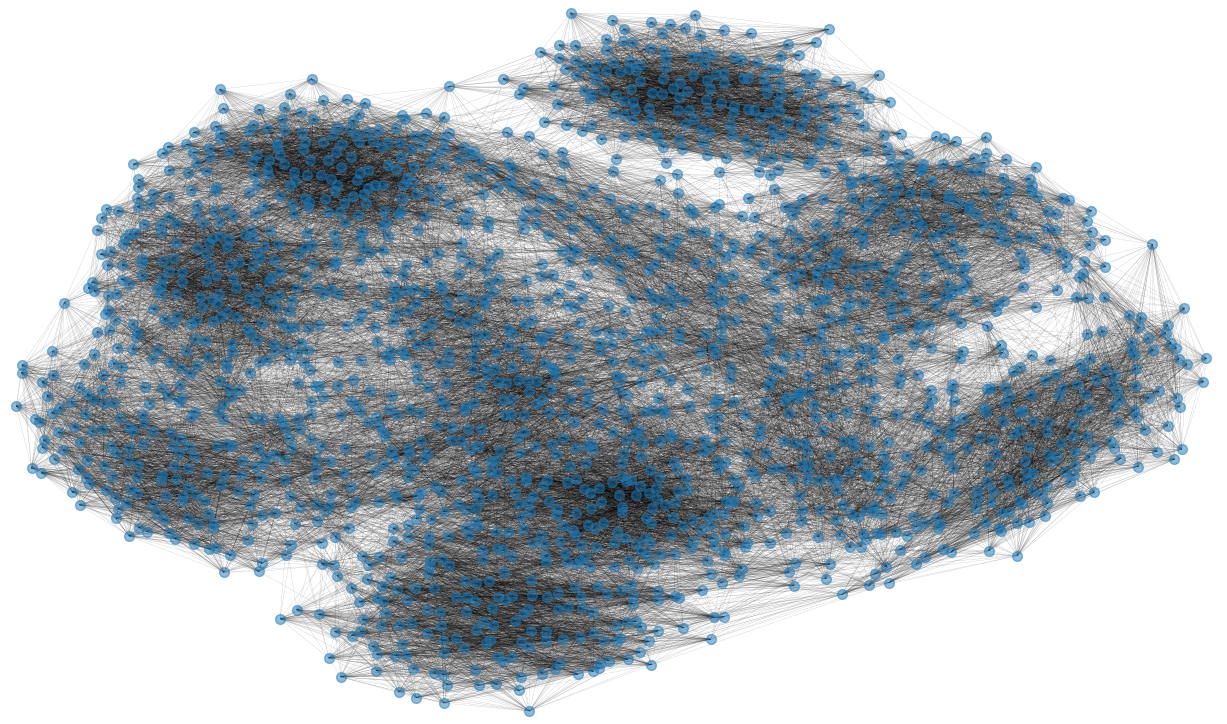
\includegraphics[scale=0.3]{./k-NNG_Kamada_OK.png}
    \caption{k-NN graph of the digits dataset for $nn = 42$ neighbors.}
\label{fig:k-NNG}
\end{figure}

The first question that arises in topological k-means is: how to build a graph from a multivariate dataset in order to create a discrete approximation to the data manifold? In graph-based machine learning, two popular methods are particularly interesting due to computational efficiency \cite{k-NNG,k-NNG2}:

\begin{enumerate}
	\item k-NN graph: for each data point $\vec{x}_i, i = 1, 2, ..., n$, we must compute the Euclidean distance to every other sample $\vec{x}_j, j \neq i, j = 1, 2, ..., n$. Then, we have to select only the $k$ samples with smallest distance (nearest neighbors) and create an edge between them.
	\item $\epsilon$-neighborhood graph: we must define a radius $\epsilon$ and for each sample $\vec{x}_i, i = 1, 2, ..., n$ and every other sample $\vec{x}_j, j \neq i, j = 1, 2, ..., n$, compute the Euclidean distance between them. For every point inside the ball of radius $\epsilon$ centered at $\vec{x}_i$, an edge must be created.
\end{enumerate}

A second question that arises is: how well the length of shortest paths in k-NN graphs can approximate the true underlying geodesic distances in the data manifold? The Asymptotic Convergence Theorem shows that, under certain regularity conditions, the length of shortest paths in k-NN graphs $d_G(\vec{x}_i, \vec{x}_j)$ converges to the geodesic distances $d_M(\vec{x}_i, \vec{x}_j)$ \cite{NIPS2002}. In summary, the authors show that the two distance metrics, $d_G(\vec{x}_i, \vec{x}_j)$ and $d_M(\vec{x}_i, \vec{x}_j)$  approximate each other arbitrarily closely, as the density of data points tends to infinity.

\vspace{0.5cm}
\begin{theorem}[Asymtptic Convergence Theorem]
	Given $\lambda_1, \lambda_2, \mu > 0$, but as small as desired, then, for a sufficiently large density of points, the following inequality holds:
	\begin{equation}
		1 - \lambda_1 \leq \frac{d_G(\vec{x}_i,\vec{x}_j)}{d_M(\vec{x}_i,\vec{x}_j)} \leq 1 + \lambda_2
	\end{equation} with probability $1 - \mu$, where $d_G(\vec{x}_i,\vec{x}_j)$ is the recovered distance (length of shortest path) and $d_M(\vec{x}_i,\vec{x}_j)$ is the true geodesic distance in the manifold.
\end{theorem}
\vspace{0.5cm}

The mathematical details of the proof can be found in the work of Bernstein and colleagues \cite{ACT}. In the following, we present the pseudo-code for the proposed topological k-means in Algorithm \ref{topkmeans_algo}.

\begin{algorithm}[H]
\caption{Topological k-means algorithm}\label{topkmeans_algo}
\begin{algorithmic}
\State // Parameters:
\State // $X$: the $n \times d$ data matrix (each row is a sample)
\State // $n$: the number of samples
\State // $k$: the number of clusters
\State // $nn$: the number of neighbors in the k-NN graph
\Function{Top-k-means}{$X, n, k, nn$}
\State $\vec{s}_1, \vec{s}_2, .., \vec{s}_k \gets select\_random\_seeds(X, k)$ \Comment{Select k random centers}
\State $distances \gets zeros(k, n)$ \Comment{Array to store the geodesic distances}
\For{$i \gets 1$; $i \leq k$; $i++$}	
	\State $\vec{\mu}_i \gets \vec{s}_i$		
\EndFor
\While{not convergence}
	\State $G \gets kNN\_Graph(X, nn)$	\Comment{Build the k-NN graph}
	\For{$i \gets 1$; $i \leq k$; $i++$}
		\State $\omega_i \gets \{ \}$		\Comment{Begin with $k$ empty partitions}
	\EndFor
	\For{$j \gets 1$; $i \leq k$; $j++$}
		\State $distances[j] \gets Dijkstra(G, \vec{\mu}_j)$  \Comment{Geodesic distances}
	\EndFor
	\For{$i \gets 1$; $i \leq n$; $i++$}
		\State $j \gets distances[:, i].argmin()$	\Comment{Select the nearest centroid}
		\State $\omega_j \gets \omega_j \cup \{ \vec{x}_i \} $	\Comment{Assign sample to the cluster}
	\EndFor
	\For{$i \gets 1$; $i \leq k$; $i++$}
		\State $\vec{\mu}_i \gets \frac{1}{\lvert \omega_i \rvert}\sum_{\vec{x} \in \omega_i} \vec{x}$ \Comment{Recalculate the centroids}
	\EndFor
\EndWhile 
\State \textbf{return} $\omega_1, \omega_2, ..., \omega_k$	
\EndFunction
\end{algorithmic}
\end{algorithm}

At this point, some comments about the algorithm should be done. First, note that, in comparison to regular k-means, topological k-means require an additional parameter $nn$, which is the number of neighbors in the k-NN graph. Alternatively, one can choose to parametrize the algorithm in terms of $\epsilon$, which is the radius that define the size of the neighborhood (ball centered in $\vec{x}_i$). Second, to correctly build the k-NN graph, at the end of each iteration, the new centers must be included in the data matrix $X$, because often they do not belong to the original data matrix. Finally, in this version of the algorithm, the center of the cluster $\omega_j$ is updated by computing the sample average of the samples assigned to it, but it is possible to compute an average over the geodesic distances, but that would require another execution of Dijkstra's algorithm inside the WHILE loop. Therefore, to reach a tradeoff between performance and computational cost, we chose to keep the sample average.

The main advantages of the proposed topological k-means over regular k-means can be summarized by two main points: 

\begin{itemize}
	\item Regular k-means uses the Euclidean distance, which means that it is ``blind'' for non-spherical clusters and quite sensitive to the presence of noise and outliers in data. With the incorporation of a graph-based geodesic distance, we intend to alleviate these limitations.	
	\item In high dimensional spaces, the discriminating power of the Euclidan distance is poor due to the complex geometry of hyperspaces. Hence, the performance of k-means and other clustering algorithms can be severely degraded in datasets for which the number of features $n$ is much larger than the number of samples $m$.
\end{itemize}

\subsection{Complexity analysis}

The computational complexity of the proposed topological k-means algorithm depends on the following variables: the number of samples $n$, the number of features $d$, the number of clusters $k$, the number of neighbors in the k-NN graph $nn$, the number of edges in the k-NN graph $m$ and the number of iterations $t$, which is often unknown.

Note that, the definition of the initial centers can be done in $O(k)$. The definition of the matrix of distances is performed in $O(kn)$, and the initial FOR loop is also $O(k)$. The analysis of the main WHILE loop reveals that: 

\begin{itemize}
	\item The k-NN graph construction can be done in $O(nd~log~n)$ using a KD-Tree. 
	\item Dijkstra's algorithm is executed $k$ times per iteration, resulting in a total cost of $O(km~log~n)$.
	\item The label assignment FOR loop has cost $O(kn)$.
	\item The computation of the new centers has cost $O(nd)$, as in the partition $\omega_1 + \omega_2 + ... + \omega_k = n$.
\end{itemize}

As the main WHILE loop is executed an unknown number of iterations $t$, the total cost of topological k-means is:

\begin{align}
	T(n) & = O(kn) + O(tnd~log~n) + O(tkm~log~n) + O(tkn) + O(tnd) \\ \nonumber
	     & = O(tnd~log~n) + O(tkm~log~n) = O(t(nd+km)log~n)
\end{align}

Therefore, topological k-means depends linearly and logarithmically in the number of samples $n$ and linearly in the number of edges of the k-NN graph $m$, which in terms of computational complexity is considered a quite efficient algorithm. 

\section{Experiments and results}

In order to test and evaluate the performance of the proposed method against regular k-means and HDBSCAN, a state-of-the-art hierarquical density based method for clustering that assumes the observed data is noisy. Three different cluster evaluation metrics (external indices) were selected to assess the performance of the algorithms: Rand index \cite{Rand1,Rand2}, normalized mutual information score \cite{Mutual} and V-measure \cite{Vmeasure}.

The first set of experiments was designed to compare the performance of the methods in real high dimensional datasets. All the selected datasets are freely available at the repository \url{www.openml.org}. Table \ref{tab:data} describes each dataset with names, number of samples $n$, number of features $m$ and number of classes $k$. Note that the majority of the datasets contains microarray data from the project GEMLeR. This project provides a collection of gene expression datasets that can be used for benchmarking gene expression oriented machine learning algorithms. They can be used for estimation of different quality metrics (e.g. accuracy, precision, area under ROC curve, etc.) for classification, feature selection or clustering algorithms. Each gene expression sample in GEMLeR repository comes from a large publicly available expO (Expression Project For Oncology) repository by International Genomics Consortium \cite{GEMLeR}.

\begin{table}[htb]
%%% Generated by mktable on Sat Dec 27 16:38:40 2008
%%% Started by papa with args: mktable accuracies.txt
\centering
\caption{Number of samples, features and classes of the selected openML datasets for the first set of experiments.}
\begin{tabular}{ccccc}
\toprule
\textbf{Number} & \textbf{Datasets}  & \textbf{\# samples} & \textbf{\# features} & \textbf{\# classes} \\
\midrule
1 & AP\_Colon\_Kidney       & 546                & 10935               & 2                \\
2 & AP\_Breast\_Kidney      & 604                & 10935               & 2                \\
3 & AP\_Breast\_Colon       & 630                & 10935               & 2                \\
4 & AP\_Colon\_Prostate     & 355                & 10935               & 2                \\
5 & AP\_Prostate\_Kidney    & 329                & 10935               & 2                \\
6 & AP\_Uterus\_Kidney      & 384                & 10935               & 2                \\
7 & AP\_Prostate\_Uterus    & 193                & 10935               & 2                \\
8 & AP\_Lung\_Uterus        & 250                & 10935               & 2                \\
9 & AP\_Ovary\_Kidney       & 458                & 10935               & 2                \\
10 & AP\_Lung\_Kidney        & 386                & 10935               & 2                \\
11 & tr11.wc                 & 414                & 6429                & 9                \\
12 & tr12.wc                 & 313                & 5804                & 8                \\
13 & tr45.wc                 & 690                & 8261                & 10               \\
14 & tr23.wc                 & 204                & 5832                & 6                \\
15 & tr31.wc                 & 927                & 10128               & 7                \\
16 & SRBCT                   & 83                 & 2308                & 4                \\
17 & pasture                 & 36                 & 22                  & 2                \\
18 & analcatdata\_authorship & 841                & 70                  & 2                \\
19 & stock                   & 950                & 9                   & 2                \\
20 & kc1-binary              & 145                & 94                  & 2                \\
\bottomrule  
\end{tabular}
\label{tab:data}
\end{table}

It is possible to note that a common feature to most datasets is that the number of features $m$ is much larger than the number of samples $n$. For example, in dataset number 7, AP\_Prostate\_Uterus, the number of features is more than 56 times the number of samples, a situation that represents a tough challenge for clustering algorithms. %Figure \ref{fig:AP} shows an illustration of the k-NN graph for this dataset, considering the parameter $nn = 14$ (number of neighbors). Note that the lack of a cluster structure is evident from the k-NN graph, indicating a complex problem.

%\begin{figure}
%	\centering
%	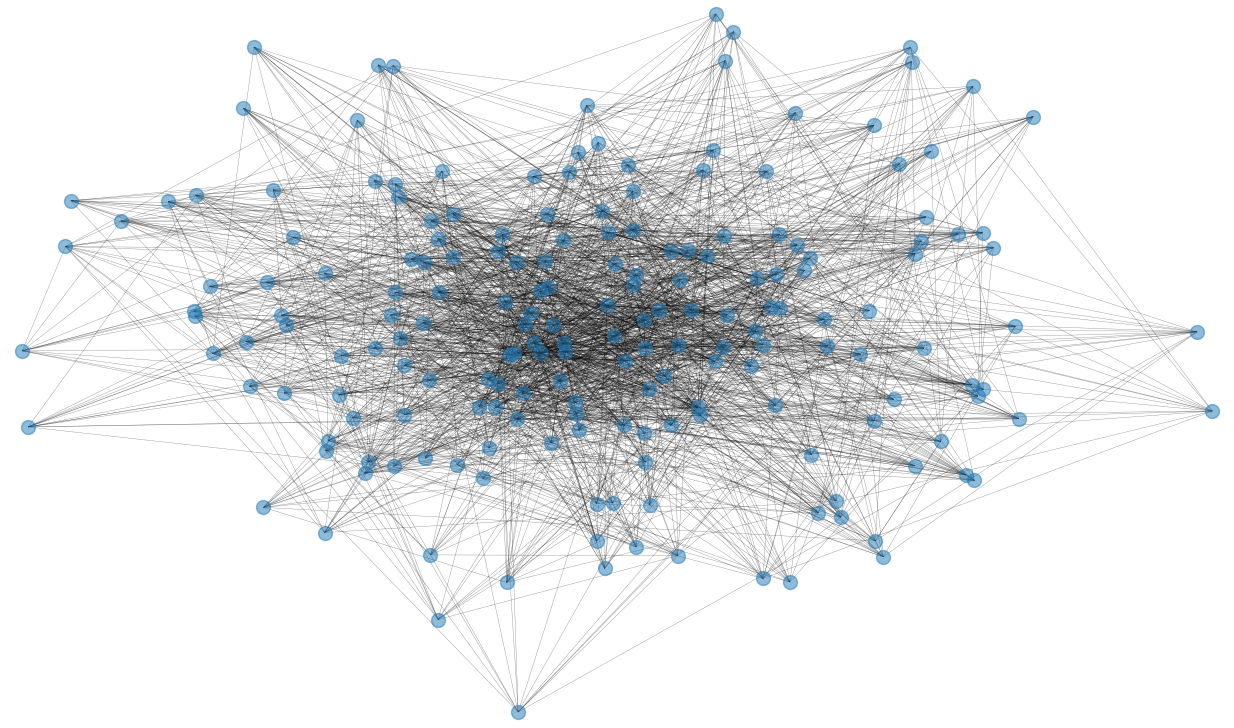
\includegraphics[scale=0.3]{./AP_Graph_OK.png}
%    \caption{k-NN graph of the AP\_Prostate\_Uterus dataset for $nn = 14$ neighbors.}
%\label{fig:AP}
%\end{figure}

The quantitative results for the clustering algorithms are presented in Table \ref{tab:results1}. Looking at the results, we see that for these datasets, the proposed topological k-means outperforms regular k-means in all three metrics. In all experiments, the parameter $k$ (number of clusters) is set equal to the number of classes and the number of neighbors $nn$ is set to $\lfloor \sqrt{n} \rfloor$. To generate the results, we computed the average performance after 30 random initializations of k-means and topological k-means. It is interesting to note that, using the standard parameter definitions, the NMI's and V-measures of HDBSCAN in the majority of these datasets are zero, because the algorithm classify all data points as noise. A possible explanation for this behavior is the sparsity of the input feature space. To check if the differences are significant, we performed a non-parametric Wilcoxon test. According to test, for a significance level $\alpha = 0.05$, there are strong evidences that the proposed topological k-means performed better than regular k-means in terms of Rand index ($p < 0.001$), normalized mutual information ($p < 0.001$) and V-measure ($p < 0.001$). 

\begin{table}[htb]
%%% Generated by mktable on Sat Dec 27 16:38:40 2008
%%% Started by papa with args: mktable accuracies.txt
\centering
\caption{Average cluster evaluation metrics obtained after 30 executions of regular k-means and topological k-means for twenty real high dimensional datasets from the openML repository.}
\begin{tabular}{ccccccc}
\toprule
 & \multicolumn{3}{c}{\textbf{Regular k-means}}               & \multicolumn{3}{c}{\textbf{Topological k-means}}        \\
\midrule
\textbf{Datasets}                & \textbf{Rand} & \textbf{NMI} & \textbf{V-meas.} & \textbf{Rand}   & \textbf{NMI}    & \textbf{V-meas.} \\
\midrule
\textbf{AP\_Colon\_Kidney}       & 0.5715        & 0.0894       & 0.1296             & \textbf{0.6970} & \textbf{0.2412} & \textbf{0.3528}    \\
\textbf{AP\_Breast\_Kidney}      & 0.5131        & 0.0116       & 0.0170             & \textbf{0.5855} & \textbf{0.1079} & \textbf{0.1620}    \\
\textbf{AP\_Breast\_Colon}       & 0.5085        & 0.0080       & 0.0118             & \textbf{0.5341} & \textbf{0.0428} & \textbf{0.0666}    \\
\textbf{AP\_Colon\_Prostate}     & 0.5074        & 0.0248       & 0.0420             & \textbf{0.6705} & \textbf{0.1585} & \textbf{0.3075}    \\
\textbf{AP\_Prostate\_Kidney}    & 0.5908        & 0.1098       & 0.2002             & \textbf{0.6682} & \textbf{0.1677} & \textbf{0.3134}    \\
\textbf{AP\_Uterus\_Kidney}      & 0.5102        & 0.0081       & 0.0122             & \textbf{0.6346} & \textbf{0.1382} & \textbf{0.2240}    \\
\textbf{AP\_Prostate\_Uterus}    & 0.5350        & 0.0461       & 0.0701             & \textbf{0.6578} & \textbf{0.2022} & \textbf{0.3096}    \\
\textbf{AP\_Lung\_Uterus}        & 0.4982        & 0.0002       & 0.0003             & \textbf{0.5500} & \textbf{0.0677} & \textbf{0.1043}    \\
\textbf{AP\_Ovary\_Kidney}       & 0.5028        & 0.0007       & 0.0016             & \textbf{0.5826} & \textbf{0.0944} & \textbf{0.1463}    \\
\textbf{AP\_Lung\_Kidney}        & 0.5761        & 0.0968       & 0.1466             & \textbf{0.6356} & \textbf{0.1369} & \textbf{0.2234}    \\
\textbf{tr11.wc}                 & 0.3571        & 0.1279       & 0.0992             & \textbf{0.5620} & \textbf{0.3875} & \textbf{0.2466}    \\
\textbf{tr12.wc}                 & 0.3046        & 0.0994       & 0.0799             & \textbf{0.4602} & \textbf{0.2757} & \textbf{0.1895}    \\
\textbf{tr45.wc}                 & 0.3947        & 0.2498       & 0.1689             & \textbf{0.5305} & \textbf{0.3617} & \textbf{0.2206}    \\
\textbf{tr23.wc}                 & 0.4331        & 0.1524       & 0.1339             & \textbf{0.5313} & \textbf{0.2076} & \textbf{0.1609}    \\
\textbf{tr31.wc}                 & 0.3650        & 0.0899       & 0.0897             & \textbf{0.4991} & \textbf{0.2064} & \textbf{0.1617}    \\
\textbf{SRBCT}                   & 0.5886        & 0.2084       & 0.1702             & \textbf{0.6193} & \textbf{0.3303} & \textbf{0.2613}    \\
\textbf{pasture}                 & 0.5254        & 0.1557       & 0.2487             & \textbf{0.6374} & \textbf{0.1941} & \textbf{0.3011}    \\
\textbf{analcatdata\_authorship} & 0.5469        & 0.1146       & 0.1780             & \textbf{0.6002} & \textbf{0.1627} & \textbf{0.2475}    \\
\textbf{stock}                   & 0.5360        & 0.0366       & 0.0530             & \textbf{0.5639} & \textbf{0.0947} & \textbf{0.1469}    \\
\textbf{kc1-binary}              & 0.5330        & 0.0326       & 0.0717             & \textbf{0.5992} & \textbf{0.1133} & \textbf{0.1723}    \\
\midrule
\textbf{Average}                 & 0.4949        & 0.0831       & 0.0962             & \textbf{0.5910} & \textbf{0.1846} & \textbf{0.2159}    \\
\textbf{Median}                  & 0.5117        & 0.0897       & 0.0848             & \textbf{0.5924} & \textbf{0.1652} & \textbf{0.2220}    \\
%\textbf{Minimum}                     & 0.3046        & 0.0002       & 0.0003             & \textbf{0.4602} & \textbf{0.0428} & \textbf{0.0666}    \\
\textbf{Maximum}                     & 0.5908        & 0.2498       & 0.2487             & \textbf{0.6970} & \textbf{0.3875} & \textbf{0.3528} \\
\bottomrule  
\end{tabular}
\label{tab:results1}
\end{table}

The second set of experiments was conducted in a different list of datasets and the main goal is to compare the performances of topological k-means and HDBSCAN (with the standard parameters) in datasets with a large number of samples and classes. Table \ref{tab:data2} describes each dataset with names, number of samples $n$, number of features $m$ and number of classes $k$. The objective here is to analyze the performance of the proposed method in datasets with a large number of high density clusters. The parameters settings for topological k-means were the same as before. For HDBSCAN, as the algorithm has a large number of parameters, we used the default configuration, that is, we used the standard parameters defined in Python's scikit-learn library, with exception of the min\_cluster\_size parameter that was set to 10. The intuiton behind this choice is to defined that a valid cluster must have at least ten data points. The optimization of HDBSCAN parameters often requires metaheuristics methods \cite{Opt}, such as genetic algorithms and particle swarm optimization, leading to a significant increase in the overall computational cost.  

\begin{table}[htb]
%%% Generated by mktable on Sat Dec 27 16:38:40 2008
%%% Started by papa with args: mktable accuracies.txt
\centering
\caption{Number of samples, features and classes of the selected openML datasets for the second set of experiments.}
\begin{tabular}{ccccc}
\toprule
\textbf{Number} & \textbf{Datasets}  & \textbf{\# samples} & \textbf{\# features} & \textbf{\# classes} \\
\midrule
1 & digits       & 1797                & 64               & 10     \\
2 & mfeat-fourier  & 2000                & 76             & 10     \\
3 & letter    & 20000             & 16                    & 26     \\
4 & mfeat-karhunen    & 355         & 64                  & 10     \\
5 & mfeat-factors    & 329          & 10935               & 10     \\
6 & optdigits      & 5620            & 64                 & 10     \\
7 & mfeat-zernike    & 2000         & 47                  & 10     \\
8 & abalone        & 4177             & 8                 & 28     \\
9 & cnae-9       & 1080              & 856                & 9      \\
10 & satimage       & 6430            & 36                & 6      \\
11 & semeion       & 1593              & 256              & 10     \\
12 & vehicle      & 846                & 18               & 4      \\
13 & micro-mass   & 360                & 1300             & 10     \\
14 & har           & 10299             & 561              & 6      \\
15 & JapaneseVowels  & 9961            & 14               & 9      \\
16 & waveform-5000   & 5000           & 40                & 3      \\
17 & texture          & 5000          & 40                & 11     \\
18 & mnist\_784 (25\%)  & 17500        & 784              & 10     \\
19 & audiology        & 226           & 69                & 24     \\
20 & yeast       & 1484               & 8                 & 10     \\
\bottomrule  
\end{tabular}
\label{tab:data2}
\end{table}


\begin{table}[htb]
%%% Generated by mktable on Sat Dec 27 16:38:40 2008
%%% Started by papa with args: mktable accuracies.txt
\centering
\caption{Average cluster evaluation metrics obtained after 30 executions of topological k-means and HDBSCAN for twenty datasets from the openML repository.}
\begin{tabular}{ccccccc}
\toprule
 & \multicolumn{3}{c}{\textbf{HDBSCAN}}                 & \multicolumn{3}{c}{\textbf{Topological Kmeans}}        \\
 \midrule
\textbf{Datasets}          & \textbf{Rand} & \textbf{NMI}     & \textbf{V-meas.} & \textbf{Rand}   & \textbf{NMI}     & \textbf{V-meas.} \\
\midrule
\textbf{digits}            & 0.7890        & 1.3493          & \textbf{0.6415}    & \textbf{0.8941} & \textbf{1.3662} & 0.6072             \\
\textbf{mfeat-fourier}     & 0.7789        & 1.0675          & \textbf{0.5454}    & \textbf{0.8682} & \textbf{1.1639} & 0.5226             \\
\textbf{letter}            & 0.7001        & \textbf{1.3258} & \textbf{0.4467}    & \textbf{0.9224} & 1.0481          & 0.3314             \\
\textbf{mfeat-karhunen}    & 0.7637        & 1.0770          & 0.5399             & \textbf{0.8880} & \textbf{1.3092} & \textbf{0.5816}    \\
\textbf{mfeat-factors}     & 0.7178        & 0.9666          & 0.4949             & \textbf{0.8744} & \textbf{1.1990} & \textbf{0.5364}    \\
\textbf{optdigits}         & 0.8027        & 1.1547          & 0.5716             & \textbf{0.8920} & \textbf{1.3177} & \textbf{0.5849}    \\
\textbf{yeast}             & 0.2539        & 0.0508          & 0.0550             & \textbf{0.7171} & \textbf{0.3515} & \textbf{0.1873}    \\
\textbf{mfeat-zernike}     & 0.6347        & 0.8764          & \textbf{0.4613}    & \textbf{0.8574} & \textbf{0.9607} & 0.4288             \\
\textbf{abalone}           & 0.6450        & 0.1622          & 0.0903             & \textbf{0.8566} & \textbf{0.4462} & \textbf{0.1605}    \\
\textbf{cnae-9}            & 0.2060        & 0.0546          & 0.0441             & \textbf{0.6842} & \textbf{0.6045} & \textbf{0.3233}    \\
\textbf{satimage}          & 0.4038        & 0.2931          & 0.2651             & \textbf{0.8007} & \textbf{0.8147} & \textbf{0.4847}    \\
\textbf{semeion}           & 0.5023        & 0.6471          & 0.3815             & \textbf{0.8525} & \textbf{0.9288} & \textbf{0.4137}    \\
\textbf{vehicle}           & 0.2864        & 0.0380          & 0.0485             & \textbf{0.6252} & \textbf{0.1977} & \textbf{0.1514}    \\
\textbf{micro-mass}        & 0.5954        & 0.5311          & 0.3278             & \textbf{0.8295} & \textbf{1.2393} & \textbf{0.5813}    \\
\textbf{har}               & 0.7129        & 0.5993          & 0.4137             & \textbf{0.8011} & \textbf{0.9570} & \textbf{0.5744}    \\
\textbf{JapaneseVowels}    & 0.1919        & 0.0828          & \textbf{0.0679}    & \textbf{0.7732} & \textbf{0.1245} & 0.0595             \\
\textbf{Waveform-5000}     & 0.3413        & 0.0016          & 0.0027             & \textbf{0.625}  & \textbf{0.2914} & \textbf{0.2813}    \\
\textbf{texture}           & 0.6017        & 0.8768          & 0.4995             & \textbf{0.8754} & \textbf{1.3268} & \textbf{0.5785}    \\
\textbf{mnist\_784 (25\%)} & 0.3586        & 0.4261          & 0.2932             & \textbf{0.8264} & \textbf{0.7737} & \textbf{0.3516}    \\
\textbf{audiology}         & 0.5825        & 0.2383          & 0.1401             & \textbf{0.8341} & \textbf{1.0736} & \textbf{0.4067}    \\
\midrule
\textbf{Average}           & 0.5434        & 0.5910          & 0.3165             & \textbf{0.8149} & \textbf{0.8519} & \textbf{0.4074}    \\
\textbf{Median}            & 0.5986        & 0.5652          & 0.3547             & \textbf{0.8433} & \textbf{0.9570} & \textbf{0.4213}    \\
%\textbf{Minimum}               & 0.1919        & 0.0016          & 0.0027             & \textbf{0.6250} & \textbf{0.1245} & \textbf{0.0595}    \\
\textbf{Maximum}               & 0.8027        & 1.3493          & 0.6415             & \textbf{0.9224} & \textbf{1.3662} & \textbf{0.6072}  \\
\bottomrule
\end{tabular}
\label{tab:results2}
\end{table}

The quantitative results for the second set of experiments are presented in Table \ref{tab:results2}. The results indicate that, in general, the proposed topological k-means outperforms HDBSCAN in the selected datasets. To check if the differences in performance are statistically significant, we performed a non-parametric Wilcoxon test. Once again, according to test, for a significance level $\alpha = 0.05$, there are strong evidences that the proposed topological k-means performed better than HDBSCAN with standard parameter settings in these datasets in terms of Rand index ($p < 0.001$), normalized mutual information ($p < 0.001$) and V-measure ($p < 0.001$). 

A few comments about the topological k-means should be addressed at this point. One important aspect about the proposed method is that we must ensure that the k-NN graph is connected, in order to allow the centers to move freely around the entire set of vertices. Otherwise, if the random initialization chooses all the centroids to be in a single connected component, the algorithm will never label the samples that belong to other connected components of $G$. There are two strategies to ensure that $G$ is connected: 1) define the  number of neighbors $nn = \lfloor \sqrt{n} \rfloor$ and while $G$ is not connected, increment $nn$ by one and build a novel k-NN graph; and 2) begin with a complete graph, extract the minimum spanning tree (MST) and add the MST edges to the k-NN graph built using $nn = \lfloor \sqrt{n} \rfloor$. Some authors argue that instead of the square root of the number of samples, a good estimative for the number of neighbors is the base two logarithm of the number of samples \cite{RandomGraphs,LOG}. However, in our experiments, $nn = log_2~n$ produced disconnected graphs for several high dimensional datasets, so we chose to consider the standard parameter configuration as $nn = \lfloor \sqrt{n} \rfloor$.

The main drawbacks of the proposed topological k-means are still related to regular k-means limitations. First, the random initialization scheme: the performance of the algorithm is directly related to the random selection of the initial centroids, something that is not under control. Better initialization strategies for k-means can be adapted to topological k-means, like k-means++ for instance \cite{kmeans++}. Methods based in topological properties of the k-NN graph can also be employed to this purpose. Another issue is related to the definition of the number of clusters $k$. In topological k-means it is possible to avoid the dependency on the parameter $k$ by estimating its value through a community detection algorithm in the k-NN graph \cite{Community}.


\section{Conclusions and final remarks}

Clustering algorithms are versatile tools in machine learning, contributing to various aspects of data analysis, exploration, and understanding. Their applications span across different domains, making them indispensable for researchers, data scientists, and analysts seeking to uncover patterns and structures within complex data. These algorithms play a crucial role in machine learning, particularly in unsupervised learning. Some examples of problems where clustering plays a major role are: pattern discovery and recognition, data exploration and understanding, anomaly detection, image and signal processing, dimensionality reduction, recommendation systems, document analysis, bioinformatics and in reducing labeling burden.

However, clustering high dimensional data still is a challenging task, especially in small sample size problems. Part of this complexity comes from the geometric properties of hyperspaces, that is, spaces with thousands of dimensions. High-dimensional data poses challenges due to the curse of dimensionality because traditional distance metrics, such as the Euclidean distance, may become less meaningful, negatively affecting the performance of clustering algorithms.

In this paper, we proposed a topological k-means algorithm that uses optimum path in graphs to approximate the true geodesic distances in the data manifold. In summary, the motivation for topological k-means was to improve the capacity of k-means to deal with high dimensional data. Overall, the main contributions of the proposed method are directly related to mitigate the the blindness of non-spherical clustering of regular k-means. Our results showed that topological k-means is capable of producing better clusters than regular k-means and even HDBSCAN, a state-of-the-art approach for data clustering. Despite being a viable and promissing algorithm, topological k-means is not perfect and has limitations. The most prominent is that the performance depends on a good initial choice of centroids, which most of the times is not under control.

In order to overcome topological k-means limitations, future works may include the development of better initialization strategies, such as the kmeans++ heuristic and a curvature-based method for sampling from data based on the shape operator. Another future improvement concerns the automatic determination of the number of clusters by means of community detection in the k-NN graph. Other strategies for graph construction can be adopted as a way to make the underlying cluster structure in data more evident, easing the work of topological k-means. Finally, the use of different metrics to weight the edges of the k-NN graph can be interesting to improve topological k-means capacity of learning different shapes of clusters.

%%===========================================================================================%%
%% If you are submitting to one of the Nature Portfolio journals, using the eJP submission   %%
%% system, please include the references within the manuscript file itself. You may do this  %%
%% by copying the reference list from your .bbl file, paste it into the main manuscript .tex %%
%% file, and delete the associated \verb+\bibliography+ commands.                            %%
%%===========================================================================================%%

\bibliography{bibliography}% common bib file
%% if required, the content of .bbl file can be included here once bbl is generated
%%\input sn-article.bbl


\end{document}
